\section{filter.h File Reference}
\label{filter_8h}\index{filter.h@{filter.h}}


This graph shows which files directly or indirectly include this file:\begin{figure}[H]
\begin{center}
\leavevmode
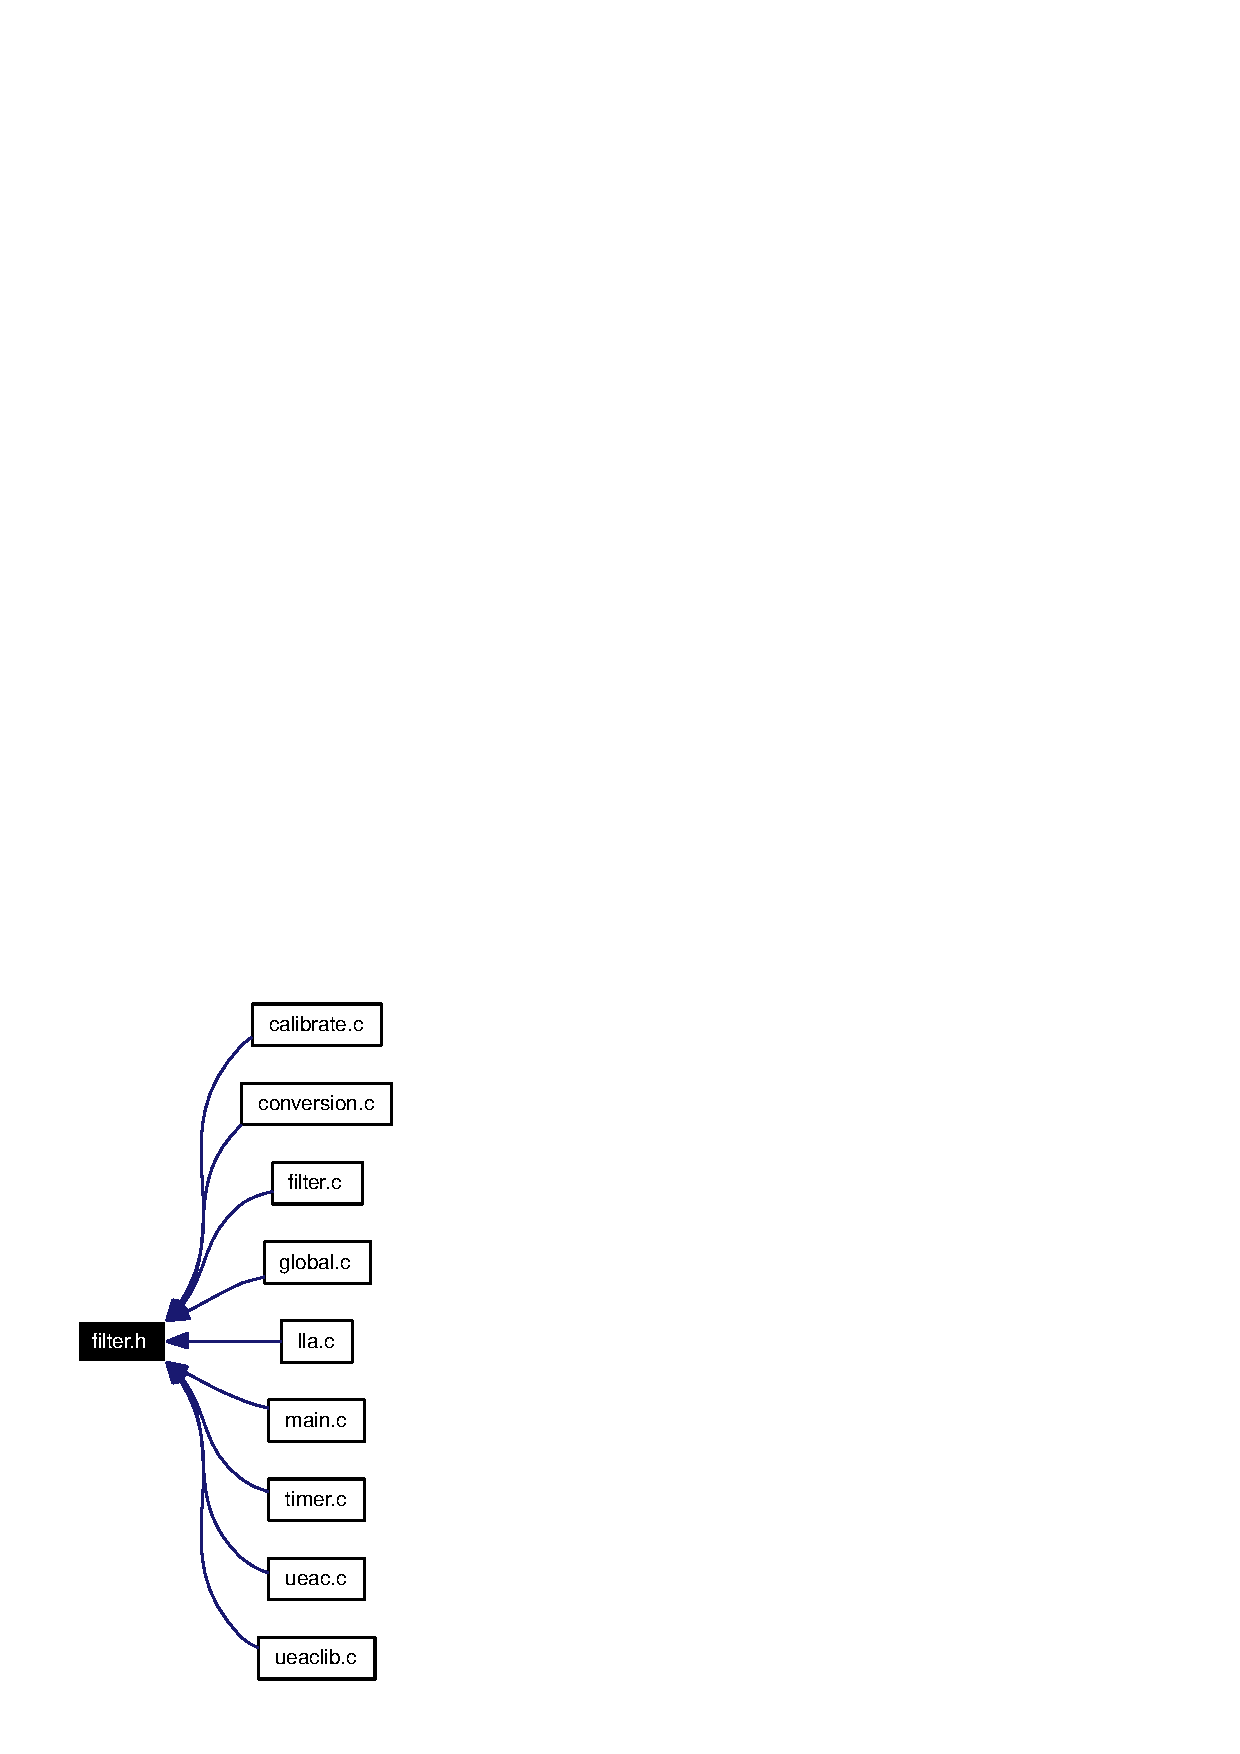
\includegraphics[width=94pt]{filter_8h__dep__incl}
\end{center}
\end{figure}
\subsection*{Data Structures}
\begin{CompactItemize}
\item 
struct {\bf channel}
\end{CompactItemize}
\subsection*{Defines}
\begin{CompactItemize}
\item 
\#define {\bf FILTER\_\-DEPTH}~16
\end{CompactItemize}
\subsection*{Typedefs}
\begin{CompactItemize}
\item 
typedef {\bf channel} {\bf channel\_\-t}
\end{CompactItemize}
\subsection*{Functions}
\begin{CompactItemize}
\item 
int {\bf initialize\_\-channel\_\-structure} ({\bf channel\_\-t} $\ast$)
\item 
unsigned short {\bf update\_\-a2d\_\-data} ({\bf channel\_\-t} $\ast$, unsigned short)
\item 
int {\bf report\_\-channel\_\-structure} ({\bf channel\_\-t} $\ast$)
\end{CompactItemize}


\subsection{Define Documentation}
\index{filter.h@{filter.h}!FILTER_DEPTH@{FILTER\_\-DEPTH}}
\index{FILTER_DEPTH@{FILTER\_\-DEPTH}!filter.h@{filter.h}}
\subsubsection{\setlength{\rightskip}{0pt plus 5cm}\#define FILTER\_\-DEPTH~16}\label{filter_8h_a0}




Definition at line 46 of file filter.h.

Referenced by initialize\_\-channel\_\-structure(), and update\_\-a2d\_\-data().

\subsection{Typedef Documentation}
\index{filter.h@{filter.h}!channel_t@{channel\_\-t}}
\index{channel_t@{channel\_\-t}!filter.h@{filter.h}}
\subsubsection{\setlength{\rightskip}{0pt plus 5cm}typedef struct {\bf channel}  {\bf channel\_\-t}}\label{filter_8h_a1}




\subsection{Function Documentation}
\index{filter.h@{filter.h}!initialize_channel_structure@{initialize\_\-channel\_\-structure}}
\index{initialize_channel_structure@{initialize\_\-channel\_\-structure}!filter.h@{filter.h}}
\subsubsection{\setlength{\rightskip}{0pt plus 5cm}int initialize\_\-channel\_\-structure ({\bf channel\_\-t} $\ast$)}\label{filter_8h_a2}




Definition at line 80 of file filter.c.

References channel::channel\_\-data, FILTER\_\-DEPTH, channel::filtered\_\-result, channel::insertion\_\-point, and channel::raw\_\-result.

Referenced by init\_\-pin\_\-data\_\-structure().

\footnotesize\begin{verbatim}80                                                             {
81   int i;
82   channel_struct->insertion_point=0;
83   for (i=0;i<FILTER_DEPTH;i++) {
84     channel_struct->channel_data[i]=0;
85   }
86   channel_struct->raw_result=0;
87   channel_struct->filtered_result=0;
88   return (0);
89 }
\end{verbatim}\normalsize 


\index{filter.h@{filter.h}!report_channel_structure@{report\_\-channel\_\-structure}}
\index{report_channel_structure@{report\_\-channel\_\-structure}!filter.h@{filter.h}}
\subsubsection{\setlength{\rightskip}{0pt plus 5cm}int report\_\-channel\_\-structure ({\bf channel\_\-t} $\ast$)}\label{filter_8h_a4}




Definition at line 65 of file filter.c.

References channel::channel\_\-data, channel::filtered\_\-result, channel::insertion\_\-point, and channel::raw\_\-result.

\footnotesize\begin{verbatim}65                                                         {
66   int i,j;
67   printf("insertion_point=%d\n",channel_struct->insertion_point);
68   printf("raw_result=%d\n",channel_struct->raw_result);
69   printf("filtered_results=%d\n",channel_struct->filtered_result);
70   for (i=0;i<4;i++) {
71     for (j=0;j<4;j++) {
72       printf("%5d ",channel_struct->channel_data[4*i+j]);
73     }
74     printf("\n");
75   }
76   printf("\n");
77   return (0);
78 }
\end{verbatim}\normalsize 


\index{filter.h@{filter.h}!update_a2d_data@{update\_\-a2d\_\-data}}
\index{update_a2d_data@{update\_\-a2d\_\-data}!filter.h@{filter.h}}
\subsubsection{\setlength{\rightskip}{0pt plus 5cm}unsigned short update\_\-a2d\_\-data ({\bf channel\_\-t} $\ast$, unsigned {\em short})}\label{filter_8h_a3}




Definition at line 49 of file filter.c.

References channel::channel\_\-data, FILTER\_\-DEPTH, channel::filtered\_\-result, channel::insertion\_\-point, and channel::raw\_\-result.

Referenced by timer\_\-a0\_\-irq().

\footnotesize\begin{verbatim}49                                                                                 {
50   long sum = 0;
51   int i;
52   channel_struct->raw_result=data;
53   channel_struct->channel_data[channel_struct->insertion_point++]=data;
54   if (channel_struct->insertion_point>=FILTER_DEPTH) {
55     channel_struct->insertion_point=0;
56   }
57   for (i=0;i<FILTER_DEPTH;i++) {
58     sum += channel_struct->channel_data[i];
59   }
60   sum /= FILTER_DEPTH;
61   channel_struct->filtered_result = (unsigned short) sum;
62   return (channel_struct->filtered_result);
63 }
\end{verbatim}\normalsize 


